\documentclass[10pt]{article}
\usepackage[a4paper,margin=22mm]{geometry}
\usepackage{graphicx,booktabs,hyperref,amsmath}
\title{Task-Specific Action Editing for Household Manipulation:\\A Six-Task Development Pilot and a Twelve-Rollout Partial Submission}
\author{Leonard Yoon\\Independent}
\date{Pre-submission research draft: 2026-10-11T10:57:18. Not submitted to arXiv.}
\begin{document}\maketitle
\begin{abstract}
We document a paired development study of frozen released manipulation policies with task-specific action editing, together with a separate partial-submission evaluation. The development panel contains 36 physical rollouts: six tasks, three instances, and two policy conditions. Mean final goal progress falls from 0.455 to 0.329 with editing, and full success falls from 5/18 to 1/18. Task 001 improves partial progress without improving full success. The final panel fixes one edited policy per task for tasks 001, 002, and 005, with four public instances each. All twelve final trials are complete, with observed mean final Q 0.224206 and full success 0/12. Missing instances count as zero in the official partial-submission score. This report supports reproducibility and failure analysis rather than a claim of general policy improvement.
\end{abstract}
\section{Scope and evidence}
BEHAVIOR-1K provides realistic household activity simulation and goal-based evaluation~\cite{behavior}. The primary evidence here is the recorded paired pilot, not a new benchmark-wide result. Development instances are native 301 (public index 0) and training instances 23 and 24. These instances were used during development and must not be represented as an untouched held-out test. The supplementary final panel is a time-constrained partial submission. The user-approved execution order is 002, 001, 005; no further research rollouts are planned after its twelve trials.
\section{Method and controls}
We use a released task-specific policy implementation~\cite{ilia}. The original actor is frozen. Task-specific auxiliary networks were trained using 20 demonstrations, 1,000 updates, batch size eight, and discount 0.999. Each condition uses seed zero for the reported panel. The action-editing configuration uses a 30-step chunk, 15 executed steps per replan, carry length four, two original proposals and one edited proposal, one edit step, and edit scale 0.01. The original wrapper retains stage voting (three predictions, two votes to promote), cross-layer KV transforms, correlated sampling, and correction rules. The online candidate path uses the encoder, edit actor, and target critic; filter critic and temperature are training components, not directly invoked for online selection. The approach is informed by action-editing and real-time policy work~\cite{expo,rt}; these citations do not establish equivalence to their full algorithms or training claims.
The paired panel reuses preserved historical baseline rollouts where recorded. It is not a prospectively randomized experiment. Capture alignment and environment/inference seeds are documented in the physical-row evidence. Different tasks use different released actors and auxiliary networks, so aggregate scores do not isolate a single universal editing effect.
\section{Paired development results}
\begin{table}[h]\centering\begin{tabular}{lrrrrr}\toprule
Task & A0 Q & RT Q & Delta Q & A0 success & RT success\\\midrule
000 & 0.667 & 0.333 & -0.333 & 2/3 & 1/3 \\
001 & 0.444 & 0.667 & +0.222 & 1/3 & 0/3 \\
002 & 0.238 & 0.143 & -0.095 & 0/3 & 0/3 \\
003 & 0.381 & 0.333 & -0.048 & 1/3 & 0/3 \\
005 & 0.444 & 0.444 & +0.000 & 1/3 & 0/3 \\
007 & 0.556 & 0.056 & -0.500 & 0/3 & 0/3 \\
\bottomrule\end{tabular}\caption{Three development instances per task and condition. Q is official final goal progress, not full task success.}\end{table}
\begin{figure}[h]\centering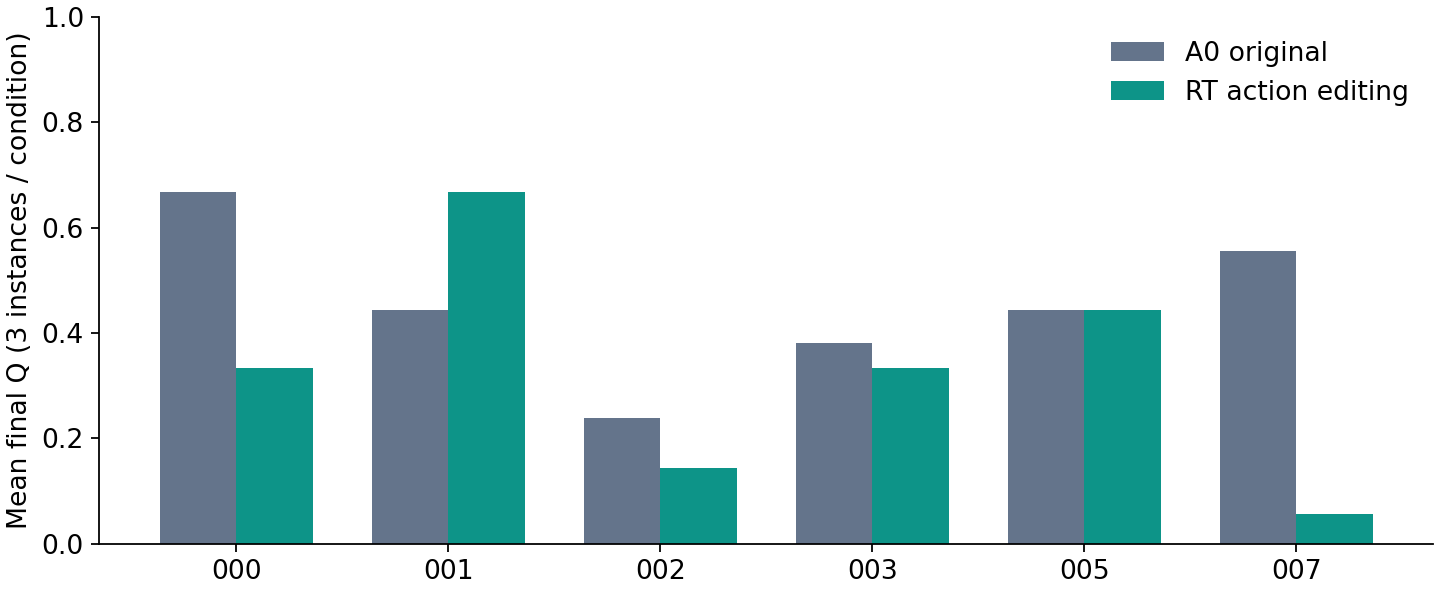
\includegraphics[width=.88\linewidth]{pilot6-Q.png}\caption{Mean final Q in the six-task paired pilot.}\end{figure}
Across 18 pairs, final Q averages 0.455 for the original actor and 0.329 for editing. Only task 001 shows a positive task-level mean Q difference (+0.222). Task 005 has approximately zero change, while task 007 decreases by 0.500. Full success decreases from five to one. Thus this configuration does not support an overall performance-improvement claim. Increasing partial progress can coexist with lower full success. Maximum intermediate Q is not interchangeable with final Q; ending predicates and retained goal satisfaction require separate video and metric inspection.
\section{Final partial-submission protocol}
The final panel contains public indices 0--3 once each for tasks 001, 002, and 005, totaling twelve trials. Native instance identifiers are 301--304. All started trials, including failures, must be retained. There is no selection of favorable repeats. Public-index-zero development exposure is disclosed; this report does not claim explicit organizer approval beyond the published protocol.
The final policy remains frozen and has five supported routes (000, 001, 002, 003, 005); the evaluated subset is three routes. Preserving unevaluated routes avoids changing the executed policy identity. The execution manifest SHA256 is \texttt{f95003a2bdb8ce6f...} (full digest in the execution manifest).
\begin{table}[h]\centering\begin{tabular}{llll}\toprule Task & Public index & Snapshot state & Final Q\\\midrule
002 & 0 & complete & 0.571 \\
002 & 1 & complete & 0.714 \\
002 & 2 & complete & 0.571 \\
002 & 3 & complete & 0.000 \\
001 & 0 & complete & 0.000 \\
001 & 1 & complete & 0.000 \\
001 & 2 & complete & 0.000 \\
001 & 3 & complete & 0.000 \\
005 & 0 & complete & 0.000 \\
005 & 1 & complete & 0.500 \\
005 & 2 & complete & 0.000 \\
005 & 3 & complete & 0.333 \\
\bottomrule\end{tabular}\caption{Final-panel status at 2026-10-11T10:57:18 UTC. All twelve reported trials are complete; none has full success.}\end{table}
\section{Runtime and reproducibility}
The clean server has four NVIDIA L40S GPUs and 46 logical CPUs. Each GPU runs a policy and simulator. Simulator CPU quotas changed from seven to ten to 10.5 without restarting active task-002 trials; later public 0/2 changed to 11 then 12, and remaining public 0/1/2 to 15 after public 3 completed. Policy quota is four. These are shared cgroup ceilings, not exclusive core reservations. Per-trial quota-change records preserve this intervention. Timing comparisons must separate steady-state rollout throughput from startup, restoration, packaging, and backup.
The pilot used a 224-pixel RGB DefaultWrapper. The final evaluator uses RGBDFullResWrapper and the unchanged R1Pro robot configuration. Input and runtime differences prevent direct attribution of pilot-to-final speed changes to hardware alone. The policy subsequently resizes RGB and does not use depth, while wrapper and simulator overhead still remain. The pinned evaluator revision is \texttt{bd049de3119acdcdf2334fe9e1ebe060fa20c108}.
L40S memory use is not evidence that the release runs on the official single-24GB-GPU setup. The user explicitly elected to skip actual 24GB hardware validation, based on approximately 20GB observed GPU usage; no additional GPU rental is planned. The embedded five-route release passed a current-L40S policy-only check with seeded reset and route switching; peak memory was 7317 MiB. Synthetic observations verify deployment, not behavior success. The image archive was uploaded and fully redownloaded at a pinned public HF revision with SHA256 verification. Registry and portal receipts are tracked separately. No additional research experiments are authorized after the twelve-trial panel.
\begin{figure}[h]\centering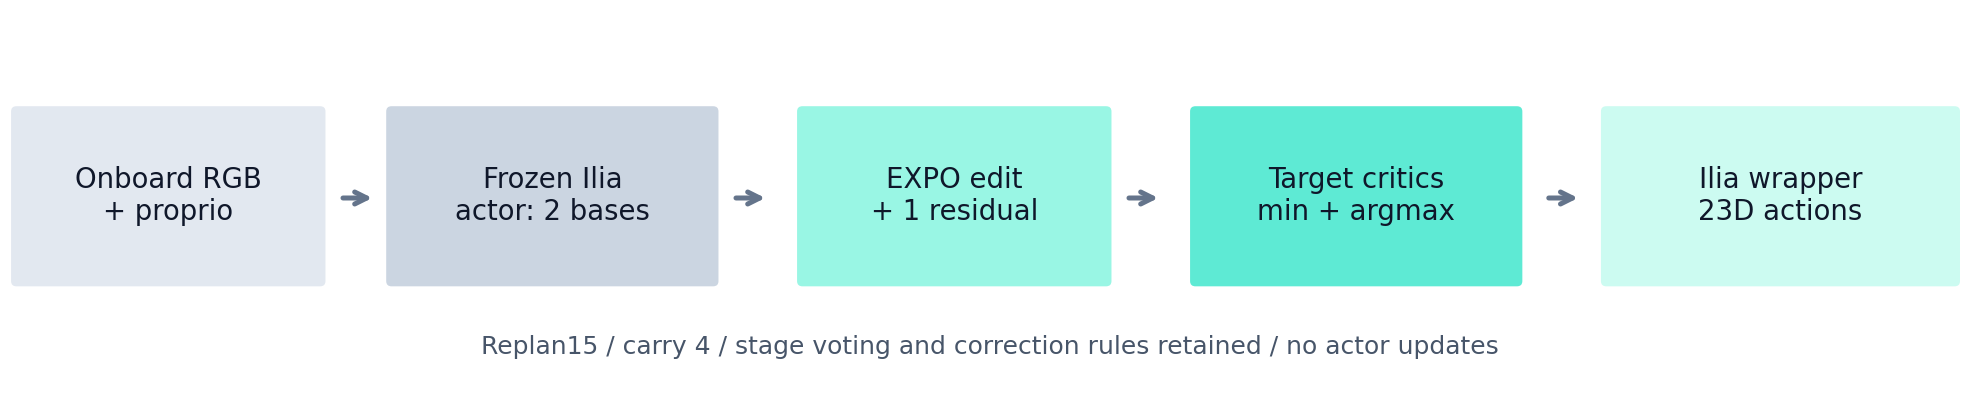
\includegraphics[width=.88\linewidth]{policy-pipeline.png}\caption{Online path: frozen actor, task-specific candidate editing, critic selection, and retained wrapper behavior.}\end{figure}
\section{Scoring and limitations}
Official partial submissions count missing instances as zero. If $q_i$ denotes each of the twelve final Q scores, the panel mean is $\sum_iq_i/12$, the selected three-task score with all ten public instances is $\sum_iq_i/30$, and the full 100-task denominator is $\sum_iq_i/1000$. For the completed panel, these values are 0.22420635, 0.08968254, and 0.00269048, respectively. Full success is0/12. The observed-panel mean must not be presented as the 1000-instance leaderboard score.
The sample is small, tasks and final scope were selected during development, simulation is nondeterministic, and there is no matched final A0 control. No significance, generalization, or benchmark leadership claim follows from this evidence. Video analysis should distinguish navigation, grasp acquisition, manipulation, placement, and goal retention while linking each observation to its original artifacts.
\section{Artifact organization and follow-up}
The main repository presents the six-task pilot, final twelve-trial status, and submission instructions. The preparation branch preserves restoration, historical scope changes, and prior experimental procedures. Submission notes remain on main until the user explicitly requests their relocation after submission. GitHub branch privacy follows repository privacy.
Private Hugging Face research and public submission catalogs separate use cases. Large historical archives remain in their original private repository with pinned revisions and SHA256 receipts. The public submission catalog contains the completed unchanged metrics, videos, release image archive, final ZIP, and reports; simulator assets, decryption keys, and credentials are excluded. Metadata audits compare archive LFS SHA256 and download the small manifest, distinct from a new full archive redownload. The final portal requires organizer-accessible assets, not merely private owner-readable URLs.
The next analysis uses preserved videos, metrics, and inference logs rather than additional research rollouts. Intermediate official goal traces were not captured. The author and affiliation were confirmed by the participant; arXiv publication has not been performed.
\begin{thebibliography}{9}
\bibitem{behavior} Chengshu Li et al.. BEHAVIOR-1K: A Human-Centered, Embodied AI Benchmark with 1,000 Everyday Activities and Realistic Simulation. 2024. \url{https://arxiv.org/abs/2403.09227}.
\bibitem{expo} Perry Dong, Kuo-Han Hung, Tian Gao, Dorsa Sadigh, and Chelsea Finn. EXPO-FT: Sample-Efficient Reinforcement Learning Finetuning for Vision-Language-Action Models. 2026. \url{https://arxiv.org/abs/2605.25477v2}.
\bibitem{rt} Perry Dong, Kuo-Han Hung, Dorsa Sadigh, and Chelsea Finn. Reinforcement Learning for Real-Time Vision-Language-Action Policies. 2026. \url{https://arxiv.org/abs/2609.18207v1}.
\bibitem{ilia} Ilia Larchenko. BEHAVIOR-1K solution: released implementation. 2025. \url{https://github.com/IliaLarchenko/behavior-1k-solution/tree/ca556f74a455cef7987a2be4537b5ac85cc56dd7}.
\end{thebibliography}\end{document}
